\begin{center}
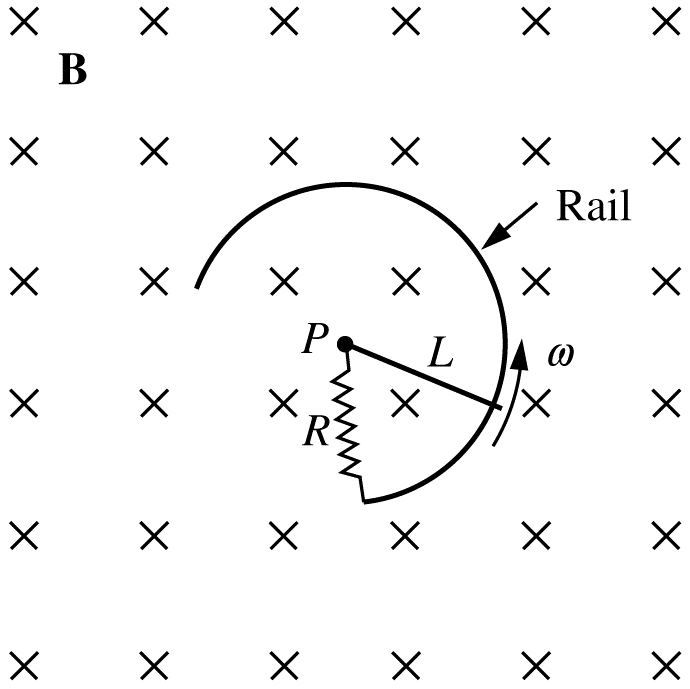
\includegraphics[scale=0.25]{images/img-007-007.png}
\end{center}

% Multiple Choice Question 11
\begin{questions}\setcounter{question}{10}\question
A conducting rod of length $L$ is pivoted at point $P$. The other end slides with negligible friction on a conducting rail in the shape of a circular arc. The plane of the rail and rod is perpendicular to a uniform magnetic field of magnitude $B$ directed into the page, as shown in the figure above. The rod rotates counterclockwise at constant angular velocity $\omega$. Assume that all the resistance of the circuit is contained in the resistor $R$. Which of the following describes the induced current in the view shown?

\begin{choices}
\choice It is counterclockwise and constant.
\choice It is counterclockwise and increasing.
\choice It is clockwise and constant.
\choice It is clockwise and increasing.
\choice It is oscillating.
\end{choices}\end{questions}

